\section{Method}
\label{sec:method}

To connect speech articulation with explicit linguistic structure, AudioMouth generates mouth-related ARKit trajectories through the three-stage pipeline in Figure~\ref{fig:overview}.
The left column summarizes the pipeline. The three modules on the right address local audio-linguistic alignment, articulatory conditioning and coefficient imbalance, and sequence-level motion supervision, respectively.
We first formulate the prediction task, then describe these modules in order; Algorithm~\ref{alg:framework} summarizes training and inference.

\begin{figure*}[h]
    \centering
    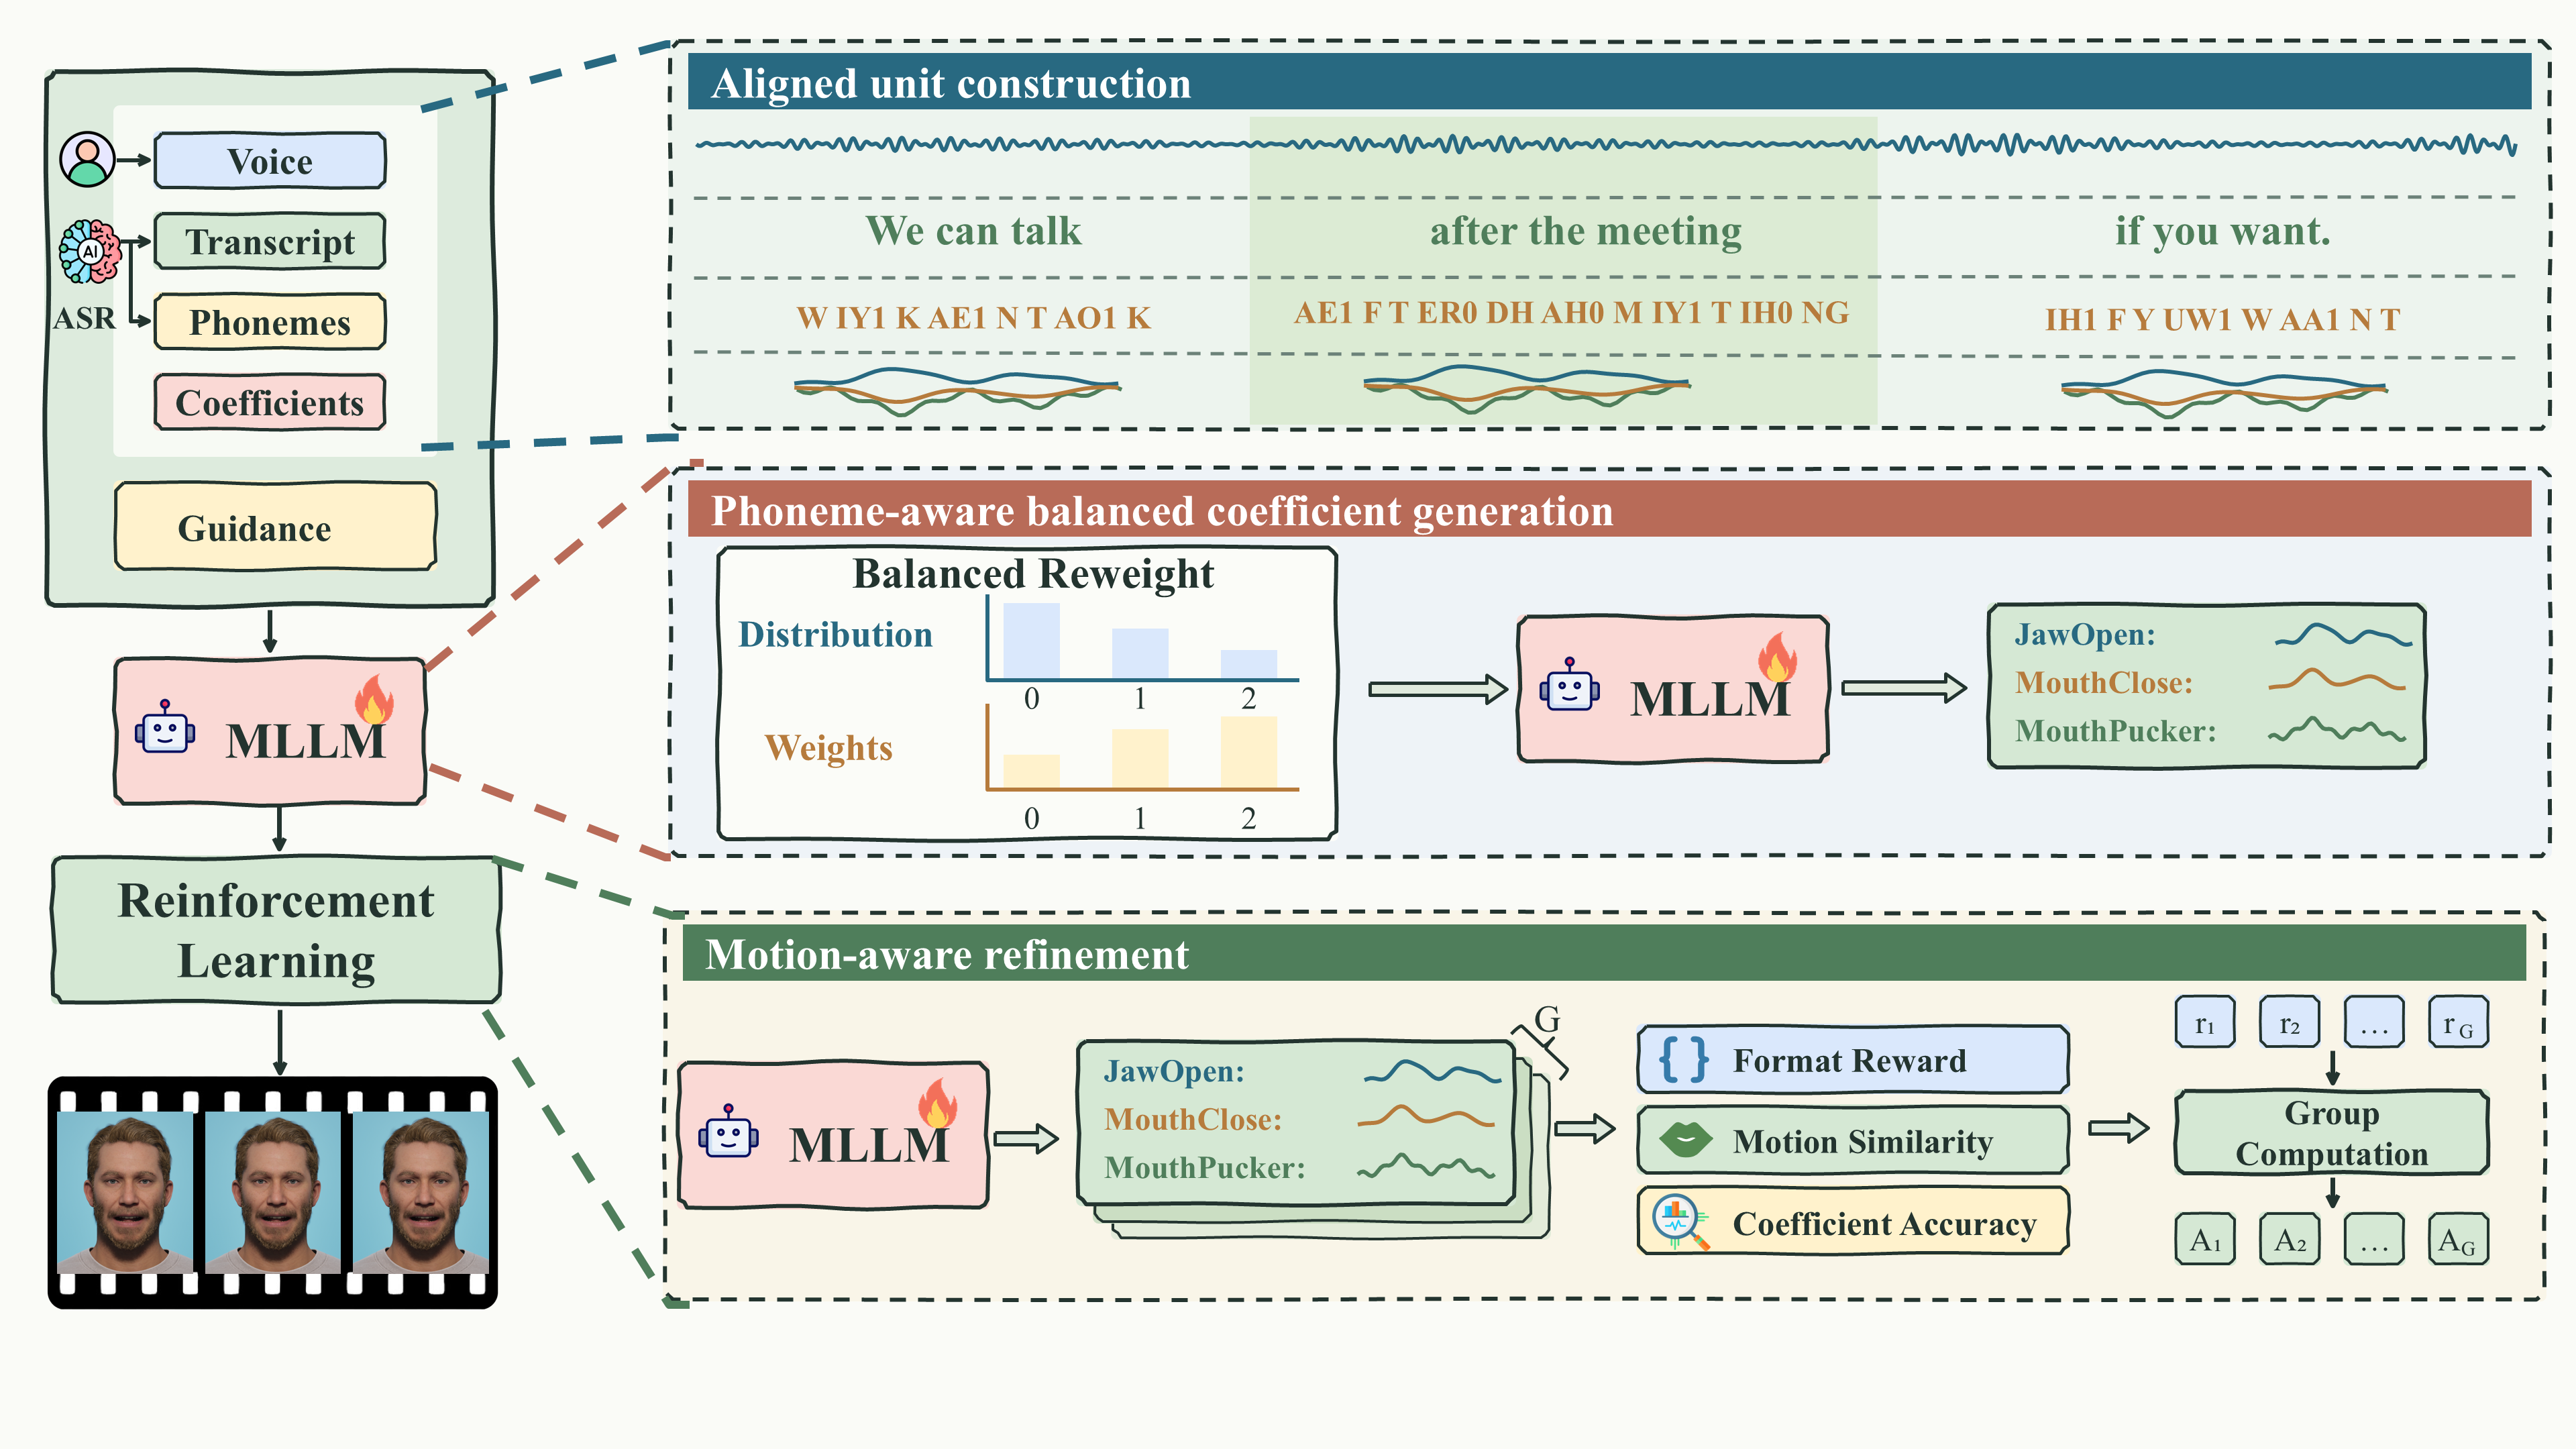
\includegraphics[width=\textwidth]{img/method.png}
    \caption{
Overview of AudioMouth. The left column shows the overall pipeline. The upper-right module constructs aligned audio-linguistic units, the middle-right module learns phoneme-aware coefficient generation with distribution-balanced supervision, and the lower-right module refines sampled sequences through group-relative policy updates using format validity and motion-quality feedback. At inference, the refined generator predicts segment-level coefficients, which are concatenated and post-processed for animation.
    }
    \label{fig:overview}
\end{figure*}

\subsection{Problem Formulation}
\label{sec:problem_formulation}

Given a speech waveform $\mathcal{A}=\{a_n\}_{n=1}^{N}$ and aligned linguistic inputs, our goal is to predict a synchronized coefficient sequence $\mathcal{V}=\{v_t\}_{t=1}^{T}$, where $v_t\in\mathbb{R}^{K}$ contains $K=32$ mouth-related ARKit controls.
Here, $N$ and $T$ denote the numbers of audio samples and motion frames, respectively; paired coefficient sequences provide supervision during training.
We divide each recording into $J$ aligned units, with segment-level inputs and targets
\[
\mathcal{X}^j=(\mathcal{A}^j,w^j,\mathcal{P}^j), \qquad
\mathcal{Y}^j=\mathrm{Serialize}_{\mathrm{json}}(\mathcal{V}^j),
\]
where $w^j$ and $\mathcal{P}^j$ are the transcript and phoneme sequence associated with audio segment $\mathcal{A}^j$, and $\mathcal{V}^j$ is its target motion.
To express motion as a structured sequence for the MLLM, we serialize each ARKit channel as a predefined JSON key with a temporally ordered sequence of coefficient values.
The MLLM models the resulting token sequence $\mathcal{Y}^j=(y_1,\ldots,y_{M_j})$ autoregressively:
\begin{equation}
p_\theta(\mathcal{Y}^j\mid\mathcal{X}^j)
=\prod_{m=1}^{M_j}p_\theta(y_m\mid y_{<m},\mathcal{X}^j),
\label{eq:structured_generation}
\end{equation}
where $\theta$ denotes the generator parameters, $M_j$ is the output token length, and $y_{<m}$ denotes the preceding tokens.
The conditioning also includes the articulation guidance described in Section~\ref{sec:stage2}, omitted from the notation for brevity.

This formulation requires local correspondence between the conditioning signals and target motion.
Moreover, frequent low-valued coefficients can dominate token-level supervision, while token likelihood alone does not measure the geometry or dynamics of a generated sequence.
The following three modules address alignment, coefficient imbalance, and motion-level supervision, respectively.

\subsection{High-Quality Audio-Linguistic Unit Construction}
\label{sec:stage1}

To preserve local correspondence between linguistic content and motion across long recordings, we construct aligned audio-linguistic units in the upper-right module of Figure~\ref{fig:overview}.
Semantic boundaries retain coherent utterances, while shared timestamps associate their speech sounds with the corresponding motion targets.

\paragraph{Semantic Segmentation and Temporal Alignment.}
For general and in-the-wild recordings, ASR provides the transcript $\tilde{W}$ and word-level timestamps $\tau$, and SAT partitions the transcript into semantically coherent segments $\mathcal{W}=\{w^j\}_{j=1}^{J}$.
The shared temporal boundaries align each audio segment $\mathcal{A}^j$ with its transcript $w^j$, associated phoneme sequence $\mathcal{P}^j$, and training motion target $\mathcal{V}^j$.
These units provide local linguistic and motion correspondence for coefficient generation. At inference, the same input construction omits the target motion.

\subsection{Phoneme-Aware Balanced Coefficient Generation}
\label{sec:stage2}

To translate the aligned linguistic cues into facial controls while reducing bias toward frequent coefficient values, we combine phoneme-aware conditioning with distribution-balanced supervision.
The middle-right module of Figure~\ref{fig:overview} implements these two components through supervised fine-tuning (SFT) of the conditional distribution in Eq.~\ref{eq:structured_generation}.

\paragraph{Phoneme-Aware Conditioning.}
To make the relationship between speech sounds and facial actions explicit, we condition the MLLM on the audio segment $\mathcal{A}^j$, transcript $w^j$, phonemes $\mathcal{P}^j$, and phoneme-to-articulation guidance.
The guidance links phonetic categories to actions such as lip closure for bilabial phonemes and larger jaw opening for open vowels, while audio supplies the acoustic evidence for the generated trajectories.

\paragraph{Distribution-Balanced Supervision.}
To prevent frequent low-valued coefficients from dominating next-token supervision, we reduce their loss contribution using a fixed coefficient-value weighting function $\omega$.
The distribution and weight plots in Figure~\ref{fig:overview} illustrate this imbalance and the corresponding reweighting.
Weights apply only to tokens representing trajectory values; schema-related tokens retain unit weight.
The training objective is
\begin{equation}
\mathcal{L}_{\mathrm{DB}} = -\sum_{m=1}^{M_j}\omega(y_m)\log p_\theta(y_m\mid y_{<m},\mathcal{X}^j).
\label{eq:db_sft}
\end{equation}
This objective balances coefficient-value supervision while preserving the output schema and conditioning inputs.
The resulting parameters $\theta_{\mathrm{SFT}}$ initialize the subsequent refinement stage.

\begin{algorithm}[t]
\caption{AudioMouth Training and Inference}
\label{alg:framework}
\small
\begin{algorithmic}[1]
\REQUIRE Paired data $\mathcal{D}$, pretrained MLLM $\theta_0$, test speech $\mathcal{A}_{\mathrm{test}}$
\ENSURE Refined generator $\theta_{\mathrm{GRPO}}$ and predicted coefficients $\hat{\mathcal{V}}$
\STATE \textbf{Aligned Unit Construction:} $\mathcal{U}\leftarrow\emptyset$
\FOR{each $(\mathcal{A},\mathcal{V})\in\mathcal{D}$}
    \STATE $(\tilde{W},\tau)\leftarrow\mathrm{ASR}(\mathcal{A})$; $\mathcal{W}\leftarrow\mathrm{SAT}(\tilde{W})$
    \STATE Add aligned units $(\mathcal{X}^j,\mathcal{V}^j,\mathcal{Y}^j)$ to $\mathcal{U}$ using Section~\ref{sec:stage1}
\ENDFOR
\STATE \textbf{Phoneme-Aware Balanced Coefficient Generation}
\STATE Set fixed coefficient-value weights $\omega$ for distribution-balanced supervision
\STATE $\theta_{\mathrm{SFT}}\leftarrow\mathrm{SFT}(\theta_0,\mathcal{U},\omega)$ using Eq.~\ref{eq:db_sft} and articulation guidance
\STATE \textbf{Motion-Aware Refinement:} $\theta\leftarrow\theta_{\mathrm{SFT}}$
\FOR{each training unit $(\mathcal{X}^j,\mathcal{V}^j,\mathcal{Y}^j)\in\mathcal{U}$}
    \STATE Sample $G$ candidates $\{\hat{\mathcal{Y}}^j_i\}_{i=1}^{G}\sim p_\theta(\cdot\mid\mathcal{X}^j)$
    \STATE Parse candidates and compute $\{r_i\}_{i=1}^{G}$ against $\mathcal{V}^j$, with validity and length handling
    \STATE $\hat{A}_i\leftarrow(r_i-\bar{r})/(\sigma_r+\epsilon)$ for each candidate
    \STATE Update $\theta$ with GRPO using $\{\hat{A}_i\}_{i=1}^{G}$ (Section~\ref{sec:stage3})
\ENDFOR
\STATE $\theta_{\mathrm{GRPO}}\leftarrow\theta$
\STATE \textbf{Inference}
\STATE Construct $\{\mathcal{X}^j\}_{j=1}^{J}$ from $\mathcal{A}_{\mathrm{test}}$ using Section~\ref{sec:stage1}
\STATE Generate $\hat{\mathcal{Y}}^j$ with $\theta_{\mathrm{GRPO}}$ and parse into $\hat{\mathcal{V}}^j$ for each unit
\STATE $\hat{\mathcal{V}}\leftarrow\mathrm{PostProcess}(\mathrm{Concat}(\{\hat{\mathcal{V}}^j\}_{j=1}^{J}))$ in temporal order
\end{algorithmic}
\end{algorithm}

\subsection{Motion-Aware Refinement}
\label{sec:stage3}

To supervise the temporal dynamics and mouth geometry that token likelihood does not directly measure, we refine the SFT generator with sequence-level motion rewards using Group Relative Policy Optimization (GRPO), as shown in the lower-right module of Figure~\ref{fig:overview}.
Starting from $\theta_{\mathrm{SFT}}$, we sample $G$ candidate JSON outputs for each input $\mathcal{X}^j$ and compare their decoded trajectories with the reference $\mathcal{V}^j$.
The reward combines coefficient accuracy, temporal dynamics, and mouth geometry for valid candidates; relative rewards within each group guide the policy update.

\paragraph{Simplified Lip-Geometry Discrepancy (SLMD).}
To capture how coefficient errors jointly affect mouth shape, we introduce SLMD, which measures their combined geometric effect through a fixed ARKit blendshape basis.
This provides geometric feedback without rendering candidate videos or detecting landmarks.
Let $\mathbf{C}^{p},\mathbf{C}^{g}\in\mathbb{R}^{T\times K}$ denote candidate and reference sequences expressed in the coefficient convention of this basis.
For each mouth-region vertex $m\in\mathcal{M}$, $\mathbf{b}_{k,m}\in\mathbb{R}^{3}$ is the displacement of the $k$-th blendshape mesh from the neutral mesh.
The shared neutral geometry cancels when comparing the two sequences, giving
\begin{align}
\delta\mathbf{x}_{t,m} &= \sum_{k=1}^{K}(c^p_{t,k}-c^g_{t,k})\mathbf{b}_{k,m}, \label{eq:slmd_displacement}\\
\mathcal{L}_{\mathrm{slmd}} &= \frac{\sum_{t=1}^{T}\sum_{m\in\mathcal{M}}w_m\|\delta\mathbf{x}_{t,m}\|_2}{T\sum_{m\in\mathcal{M}}w_m}. \label{eq:slmd}
\end{align}
Here, $T$ denotes the compared segment length, and the fixed vertex weights $w_m$ emphasize the lips while retaining lower-weight surrounding vertices.
SLMD is thus a weighted mean Euclidean discrepancy in 3D mouth deformation; the basis and weights are reused across candidates.
It supplies a geometric training signal distinct from the rendered-video 2D landmark distance used for evaluation.

\paragraph{Motion-Level Reward.}
To assess both mouth shape and its evolution over time, we combine SLMD with coefficient MSE and first- and second-order temporal difference discrepancies, denoted by $\mathcal{L}_{\mathrm{mse}}$, $\mathcal{L}_{\mathrm{vel}}$, and $\mathcal{L}_{\mathrm{acc}}$.
The temporal terms compare motion changes with the reference rather than penalizing movement itself.
To account for their different numerical scales, each discrepancy is converted into a bounded score before aggregation:
\begin{align}
S_q &= \left(1+\mathcal{L}_q/s_q\right)^{-1}, \label{eq:normalized_score}\\
r_{\mathrm{motion}} &= \sum_{q\in\{\mathrm{mse},\mathrm{vel},\mathrm{acc},\mathrm{slmd}\}}\lambda_q S_q. \label{eq:motion_reward}
\end{align}
The scales $s_q$ are fixed reference medians, and the nonnegative weights $\lambda_q$ sum to one.
Valid candidates receive the motion reward with a length-mismatch penalty when applicable; invalid outputs receive fixed negative penalties.
These operations correspond to the coefficient-accuracy, motion-similarity, and format-reward blocks in Figure~\ref{fig:overview}.

\paragraph{Group-Relative Policy Update.}
To favor higher-quality motion among candidates generated for the same input, we convert their rewards $\{r_i\}_{i=1}^{G}$ into group-relative advantages $\hat{A}_i=(r_i-\bar{r})/(\sigma_r+\epsilon)$, where $\bar{r}$ and $\sigma_r$ are the group mean and standard deviation, and $\epsilon$ ensures numerical stability.
The group-computation block in Figure~\ref{fig:overview} supplies these advantages to the GRPO policy update.
The resulting generator $\theta_{\mathrm{GRPO}}$ retains the structured output representation learned during SFT and is further optimized using motion-level feedback.

\paragraph{Inference.}
Given test speech, we construct the aligned input units and use $\theta_{\mathrm{GRPO}}$ to generate a JSON coefficient sequence for each segment.
To reconstruct a complete trajectory and reduce discontinuities between segments, we concatenate the decoded predictions in temporal order and apply post-processing, completing the pipeline in the left column of Figure~\ref{fig:overview}.
%标题需要把创新的位置推出来
%总页数9页，需要进一步压缩
%标注图采用纵向排版，才用左边一列讲述流程，然后右边一列拉开来细讲
%公式可以全部摆在一行内
